\chapter{Sekilas Evolusi Manusia}\label{ch:g12:human-evolution}

Dalam lapisan abu vulkanik berumur tiga setengah juta tahun, dua jejak
tapak kaki berjalan bersisian sepanjang dua puluh tujuh meter. Jejak
itu ditinggalkan oleh makhluk yang berjalan tegak, tumit lebih dahulu,
dengan telapak melengkung dan ibu jari kaki sejajar dengan jari
lainnya --- kaki seperti kaki kita --- pada masa ketika belum ada otak
yang lebih besar daripada otak kera. Berjalan tegak datang lebih dulu,
dua juta tahun lebih awal; otak, perkakas dan tutur kata datang
kemudian, bukan dalam satu garis lurus melainkan sepanjang sebuah
semak \omterm{def:g10:biodiversity-scales:species}{spesies}, yang sebagian besar tak meninggalkan keturunan. Bab ini
menerapkan alat dua bab terakhir --- karakter bersama, pohon, tarikh,
\omterm{def:g10:universal-dna:information}{DNA} --- pada garis keturunan yang berujung pada kita.

\section{Manusia di antara primata}

\begin{proposition}[Tempat kita pada pohon]\label{prop:g12:human-evolution:place}
Manusia adalah primata: mamalia dengan tangan yang dapat menggenggam,
kuku alih-alih cakar, \omterm{def:g11:the-eye:parts}{mata} yang menghadap ke depan dan otak yang besar
bagi ukurannya. Di dalam primata, kera besar --- orangutan, gorila,
simpanse, bonobo, manusia --- membentuk sebuah \omterm{prop:g12:phylogenetic-trees:rules}{klad}, dan di dalamnya
simpanse dan bonobo adalah kelompok saudari manusia: \omterm{def:g10:universal-dna:information}{DNA} kita berbeda
dari \omterm{def:g10:universal-dna:information}{DNA} mereka pada sekitar 1.2\% posisi, dan nenek moyang bersama
kedua garis keturunan itu hidup kira-kira enam sampai tujuh juta tahun
lalu, di Afrika. Nenek moyang itu bukan simpanse dan bukan pula
manusia; kedua garis keturunan telah berevolusi sejak saat itu.
\end{proposition}
\begin{proof}[Bukti percobaan]
Matriks karakter dan perbandingan \omterm{def:g10:universal-dna:information}{DNA} pada
\cref{ch:g12:phylogenetic-trees}: setiap \omterm{def:g10:universal-dna:gene}{gen} yang diurutkan
menempatkan simpanse lebih dekat kepada manusia daripada kepada
gorila, dan \omterm{def:g11:cell-cycle-mitosis:chromosome}{kromosom} 2 manusia adalah peleburan, ujung ke ujung, dua
\omterm{def:g11:cell-cycle-mitosis:chromosome}{kromosom} yang tetap terpisah pada simpanse --- itulah sebabnya kita
punya 23 pasang dan mereka 24. Jam molekuler, yang dikalibrasi pada
tarikh fosil pemisahan primata yang lebih tua, memberi tarikh bagi
simpul manusia--simpanse.
\end{proof}

\begin{definition}[Garis keturunan manusia]\label{def:g12:human-evolution:lineage}
\emph{Garis keturunan manusia}\index{garis keturunan manusia} adalah
\omterm{prop:g12:phylogenetic-trees:rules}{klad} semua \omterm{def:g10:biodiversity-scales:species}{spesies} yang lebih dekat kepada manusia modern daripada
kepada simpanse: segala sesuatu yang turun dari sisi manusia pada
simpul berumur enam juta tahun itu. \omterm{prop:g12:phylogenetic-trees:rules}{Klad} ini memuat satu \omterm{def:g10:biodiversity-scales:species}{spesies} yang
masih hidup, \emph{Homo sapiens}, dan sekitar dua puluh \omterm{def:g10:biodiversity-scales:species}{spesies} fosil
--- para australopitesin dan beberapa \omterm{def:g10:biodiversity-scales:species}{spesies} marga \emph{Homo}.
Sebuah fosil termasuk di dalamnya bila menunjukkan karakter turunan
garis keturunan itu: berjalan tegak, wajah yang memendek, taring yang
kecil, dan kemudian otak besar serta perkakas.
\end{definition}

\section{Karakter garis keturunan itu}

\begin{proposition}[Bipedalisme datang lebih dulu]\label{prop:g12:human-evolution:bipedalism}
Karakter turunan paling awal \omterm{def:g12:human-evolution:lineage}{garis keturunan manusia} adalah kebiasaan
berjalan dengan dua kaki. Ia tampak pada rangkanya: lubang di dasar
tengkorak tempat sumsum tulang belakang lewat terletak di bawah
tengkorak dan bukan di belakangnya, sehingga kepalanya seimbang di
atas tulang belakang yang tegak; tulang belakangnya berlengkung ganda;
panggulnya pendek dan berbentuk mangkuk; tulang pahanya menyudut ke
dalam menuju lutut, membawa kaki ke bawah pusat tubuh; telapaknya
melengkung dengan ibu jari sejajar dengan jari lain, dibuat untuk
menolak, bukan untuk menggenggam. Semuanya sudah ada, disertai
beberapa ciri kera, pada fosil berumur empat juta tahun yang otaknya
tak lebih besar daripada otak simpanse.
\end{proposition}
\begin{proof}[Bukti percobaan]
Jejak tapak kaki dalam abu vulkanik, berumur 3.6 juta tahun,
menunjukkan langkah panjang dengan tumit menyentuh lebih dahulu dan
telapak melengkung. Rangka seekor australopitesin betina berumur 3.2
juta tahun, yang 40\% lengkap, punya panggul dan lutut mirip manusia
serta otak sekitar \qty{400}{cm^3}. Dasar tengkorak seumur itu punya
lubang sumsum di depan, di bawah tengkoraknya. Karakternya muncul
berurutan: berjalan, lalu, lebih dari sejuta tahun kemudian,
pertumbuhan otaknya.
\end{proof}

\begin{omfigure}
\begin{tikzpicture}
  \node[anchor=south west, inner sep=0] (img) at (0,0)
    {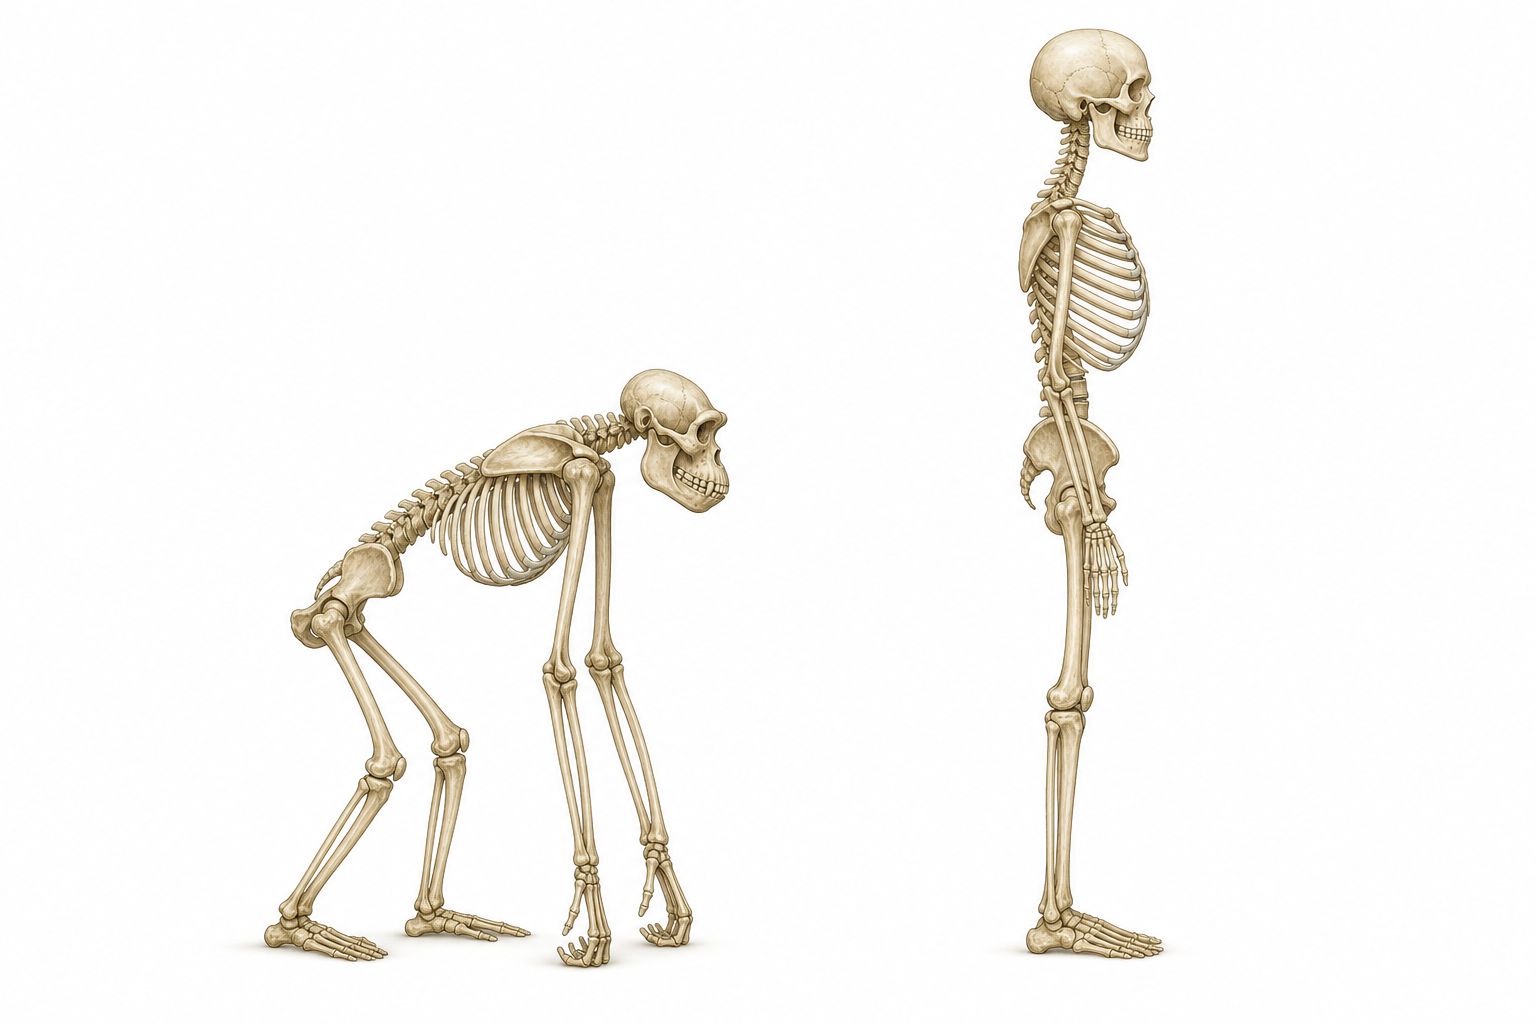
\includegraphics[width=0.56\linewidth]{images/book2/ai/fig-posture-skeletons.png}};
  \begin{scope}[x={(img.south east)}, y={(img.north west)},
      every node/.style={font=\scriptsize}]
    \draw[omDef, thick] (0.42,0.585) -- (0.42,0.98) node[above, align=center] {simpanse: lubang sumsum\\ di belakang tengkorak};
    \draw[omDef, thick] (0.29,0.50) -- (-0.03,0.62) node[left, align=right] {tulang belakang\\ miring, kepala\\ menggantung ke depan};
    \draw[omDef, thick] (0.23,0.42) -- (-0.03,0.40) node[left, align=right] {panggul panjang\\ dan sempit};
    \draw[omDef, thick] (0.25,0.26) -- (-0.03,0.18) node[left, align=right] {pinggul dan lutut\\ menekuk};
    \draw[omDef, thick] (0.70,0.86) -- (1.03,0.90) node[right, align=left] {manusia: lubang\\ sumsum di bawah\\ tengkorak};
    \draw[omDef, thick] (0.68,0.71) -- (1.03,0.68) node[right, align=left] {tulang belakang tegak\\ berlengkung ganda};
    \draw[omDef, thick] (0.70,0.54) -- (1.03,0.48) node[right, align=left] {panggul pendek\\ seperti mangkuk};
    \draw[omDef, thick] (0.69,0.32) -- (1.03,0.26) node[right, align=left] {lutut di bawah\\ batang tubuh};
  \end{scope}
\end{tikzpicture}

{\small Rangka seekor simpanse dan seorang manusia tampak samping.
Pada kera, sumsum tulang belakang keluar dari tengkorak di belakang
dan kepalanya menggantung ke depan dari tulang belakang yang miring,
di atas pinggul dan lutut yang menekuk; pada makhluk berkaki dua,
lubangnya ada di bawah tengkorak, kepalanya seimbang di atas tulang
belakang tegak berlengkung ganda, panggulnya pendek seperti mangkuk
dan lututnya berdiri di bawah batang tubuh. Dasar tengkorak, panggul
atau lutut sebuah fosil dapat dibaca untuk mengetahui cara jalannya.}
\end{omfigure}

\begin{omfigure}
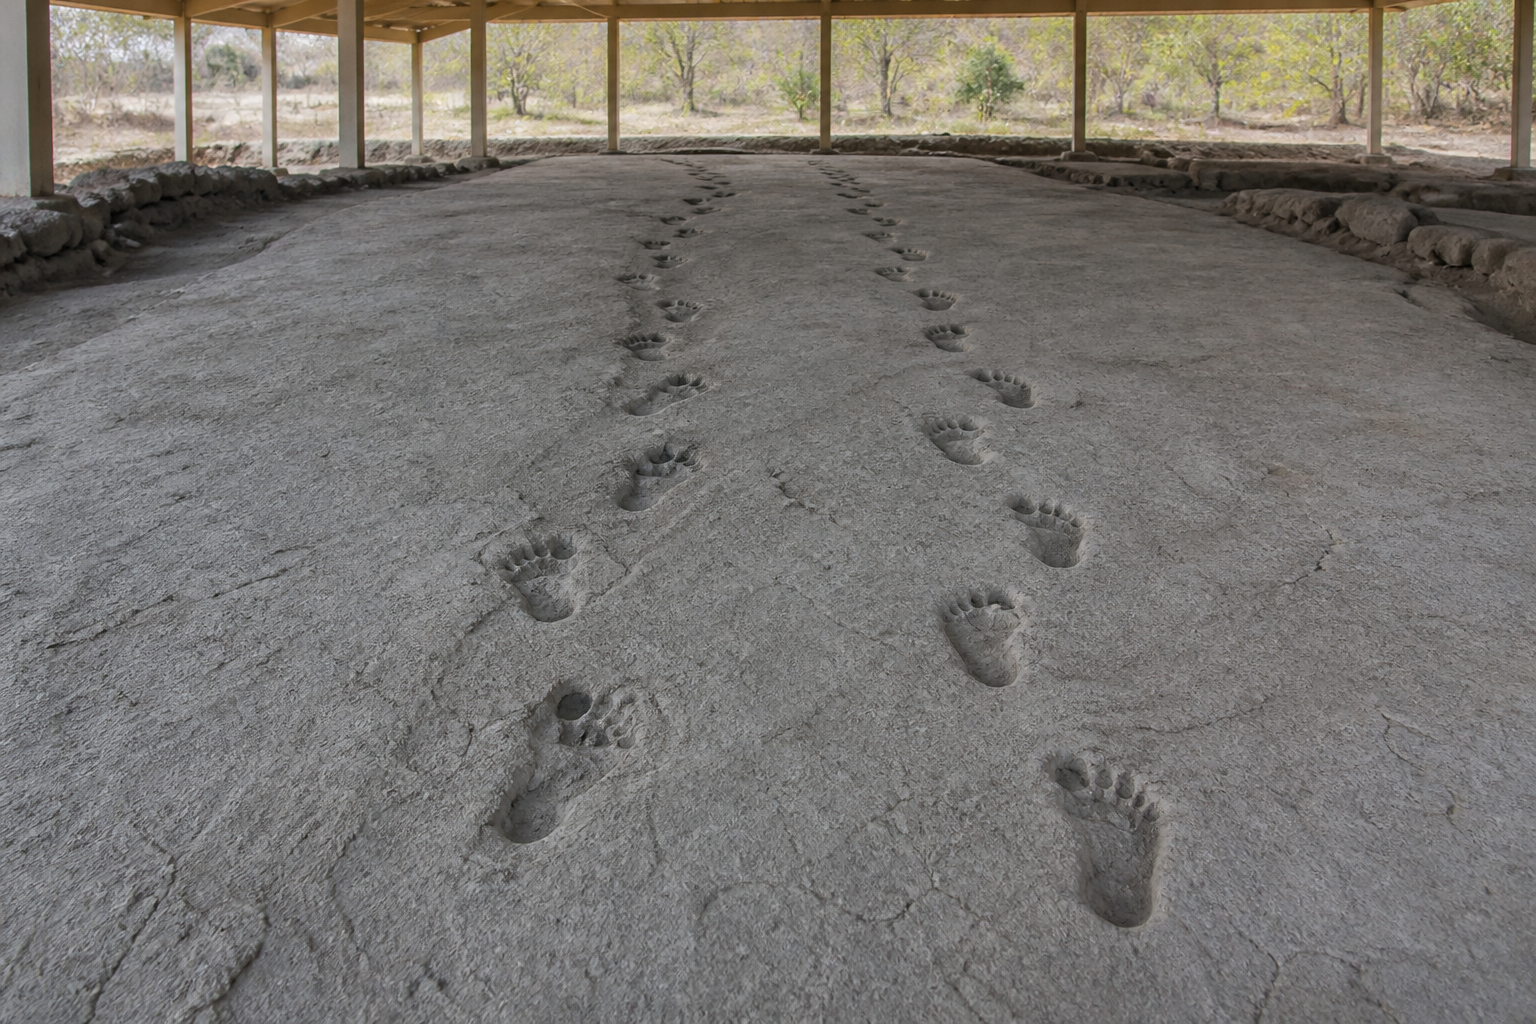
\includegraphics[width=0.6\linewidth]{images/book2/ai/g12-human-footprints.png}

{\small Sederet jejak tapak kaki yang terawetkan dalam abu vulkanik
yang mengeras. Tumit dahulu, telapak melengkung, ibu jari sejajar:
cetakan seorang pejalan tegak, dibuat jutaan tahun sebelum perkakas
batu yang pertama.}
\end{omfigure}

\begin{proposition}[Lalu otak, perkakas, dan wajahnya]\label{prop:g12:human-evolution:brain}
Sejak sekitar 2.5 juta tahun lalu garis keturunan itu menunjukkan
seperangkat karakter turunan kedua: otak yang tumbuh dari
\qty{450}{cm^3} menjadi \qty{1350}{cm^3}, wajah dan rahang yang
menyusut di bawahnya, sebuah dagu, dan perkakas batu --- mula-mula
kerakal yang diserpih hingga bermata tajam, lalu kapak genggam yang
dibentuk, lalu bilah, mata tombak dan perkakas bergagang. Api sudah
dikuasai sejuta tahun lalu, jenazah sudah dikubur seratus ribu tahun
lalu, dan gambar sudah dilukis empat puluh ribu tahun lalu. Otak dan
perkakas tumbuh bersama, masing-masing membuat yang lain berguna,
selama dua juta tahun.
\end{proposition}
\admitted

\begin{omfigure}
\begin{tikzpicture}
\begin{axis}[
  width=0.9\linewidth, height=6cm,
  axis x line=bottom, axis y line=left,
  x dir=reverse, xmin=0, xmax=4.2, ymin=300, ymax=1600,
  xlabel={juta tahun lalu}, ylabel={volume otak ($\mathrm{cm^3}$)},
  xlabel style={font=\small, at={(axis description cs:0.5,-0.12)}, anchor=north},
  ylabel style={font=\small},
  tick label style={font=\small}, xtick={4,3,2,1,0}, ytick={400,800,1200,1600},
  clip=false,
]
\addplot[only marks, mark=*, mark size=2.2pt, omThm] coordinates
  {(3.5,420) (2.5,450) (2.0,600) (1.5,850) (0.8,1000) (0.4,1250) (0.1,1450) (0.05,1350)};
\node[font=\scriptsize, anchor=south] at (axis cs:3.5,450) {australopitesin};
\node[font=\scriptsize, anchor=north] at (axis cs:2.0,570) {\emph{H. habilis}};
\node[font=\scriptsize, anchor=south] at (axis cs:1.5,880) {\emph{H. erectus} awal};
\node[font=\scriptsize, anchor=north] at (axis cs:0.8,970) {\emph{H. erectus} akhir};
\node[font=\scriptsize, anchor=south] at (axis cs:0.5,1280) {\emph{H. heidelbergensis}};
\node[font=\scriptsize, anchor=east] at (axis cs:0.12,1470) {Neanderthal};
\node[font=\scriptsize, anchor=north] at (axis cs:0.05,1320) {\emph{H. sapiens}};
\draw[dashed, gray] (axis cs:4.2,400) -- (axis cs:0,400);
\node[font=\scriptsize, gray, anchor=south east] at (axis cs:0.05,405) {simpanse (kini)};
\end{axis}
\end{tikzpicture}

{\small Volume otak \omterm{def:g10:biodiversity-scales:species}{spesies} \omterm{def:g12:human-evolution:lineage}{garis keturunan manusia} terhadap umurnya
(rerata yang dibulatkan). Datar pada \qty{400}{cm^3} khas kera selama
dua juta tahun pertama berjalan tegak, lalu melipat tiga dalam dua
juta tahun berikutnya; otak Neanderthal sedikit lebih besar daripada
otak kita.}
\end{omfigure}

\begin{omfigure}
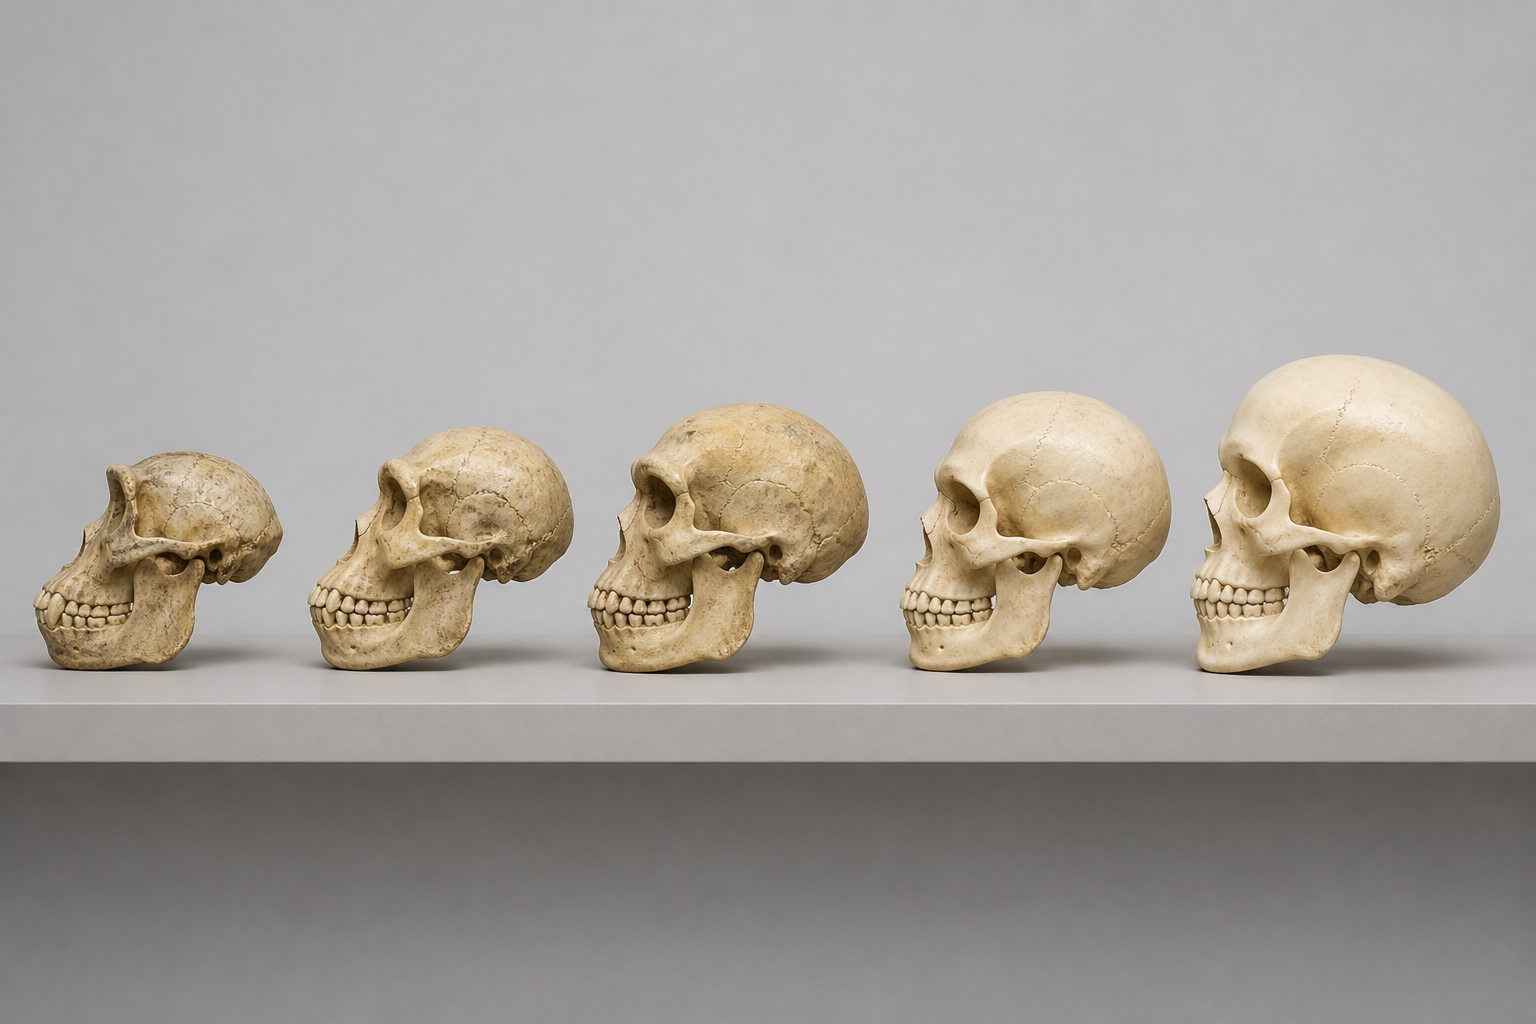
\includegraphics[width=0.66\linewidth]{images/book2/ai/g12-human-skulls.png}

{\small Tengkorak garis keturunan itu tampak samping, dari seekor
australopitesin sampai manusia modern: batok otaknya menggembung,
wajahnya mundur ke bawahnya, tonjolan alisnya memudar dan sebuah dagu
muncul.}
\end{omfigure}

\begin{example}[Membaca sebuah tengkorak]\label{ex:g12:human-evolution:skull}
Sebuah tengkorak fosil dengan lubang sumsum di bawah, batok otak
\qty{450}{cm^3}, rahang besar dan wajah menonjol adalah seekor
australopitesin: tegak, berotak kecil. Tengkorak dengan
\qty{900}{cm^3}, tonjolan alis tebal, dahi yang melandai dan tanpa
dagu adalah \emph{Homo erectus}. Tengkorak dengan \qty{1400}{cm^3},
dahi tinggi, wajah kecil yang terselip di bawah batok otak dan sebuah
dagu adalah manusia modern. Urutan karakter ini pada pohon adalah
urutan kemunculannya di dalam batuan.
\end{example}

\section{Sebuah semak, bukan tangga}

\begin{proposition}[Beberapa spesies sekaligus]\label{prop:g12:human-evolution:bush}
\omterm{def:g12:human-evolution:lineage}{Garis keturunan manusia} bukanlah satu garis nenek moyang dan keturunan
melainkan sebuah semak \omterm{def:g10:biodiversity-scales:species}{spesies}, beberapa di antaranya hidup pada waktu
yang sama: dua atau tiga macam australopitesin dua juta tahun lalu di
samping \emph{Homo} yang pertama; \emph{Homo erectus} menyebar ke tiga
benua sementara \omterm{def:g10:biodiversity-scales:species}{spesies} lain muncul di Afrika; dan baru lima puluh
ribu tahun lalu, manusia modern berbagi Bumi dengan Neanderthal di
Eropa, sebuah \omterm{def:g12:selection-drift-speciation:population}{populasi} lain di Asia, dan sebuah \omterm{def:g10:biodiversity-scales:species}{spesies} bertubuh kecil
di sebuah pulau. Sebagian besar cabang semak itu berakhir dengan
kepunahan; cabang kitalah yang tersisa.
\end{proposition}
\begin{proof}[Bukti percobaan]
Fosil \omterm{def:g10:biodiversity-scales:species}{spesies} yang berbeda ditemukan dalam lapisan seumur di situs
yang sama. Sisa Neanderthal dan manusia modern tumpang tindih di Eropa
selama beberapa ribu tahun. \omterm{def:g10:universal-dna:information}{DNA} Neanderthal dan \omterm{def:g10:universal-dna:information}{DNA} \omterm{def:g12:selection-drift-speciation:population}{populasi} Asia itu,
yang dipulihkan dari tulangnya, berbeda dari \omterm{def:g10:universal-dna:information}{DNA} kita --- dan hadir di
dalam kita: orang di luar Afrika membawa sekitar 2\% \omterm{def:g10:universal-dna:information}{DNA} Neanderthal,
dan sebagian \omterm{def:g12:selection-drift-speciation:population}{populasi} Pasifik membawa beberapa persen \omterm{def:g10:universal-dna:information}{DNA} \omterm{def:g12:selection-drift-speciation:population}{populasi}
Asia itu, yaitu jejak perkawinan silang ketika kedua \omterm{def:g10:biodiversity-scales:species}{spesies} bertemu.
Cabang-cabangnya bersentuhan sebelum berakhir.
\end{proof}

\begin{omfigure}
\begin{tikzpicture}[font=\small]
  \tikzset{bar/.style={line width=6pt, line cap=butt}}
  % time axis: 0 at right, 4 Ma at left; 3 cm per Ma
  \draw[->, thick] (0,-0.4) -- (12.6,-0.4);
  \foreach \t/\l in {0/{4}, 3/{3}, 6/{2}, 9/{1}, 12/{0}} { \draw (\t,-0.3) -- (\t,-0.5); \node[anchor=north, font=\scriptsize] at (\t,-0.55) {\l}; }
  \node[anchor=north, font=\scriptsize] at (6.3,-0.95) {juta tahun lalu};
  % species bars: (start, end) in Ma -> x = (4 - Ma)*3
  \draw[bar, omDef!60] (0.3,0.4) -- (3.3,0.4); \node[anchor=west, font=\scriptsize] at (3.4,0.4) {\emph{Australopithecus afarensis}};
  \draw[bar, omDef!60] (2.1,1.0) -- (5.7,1.0); \node[anchor=west, font=\scriptsize] at (5.8,1.0) {\emph{A. africanus}};
  \draw[bar, omDef!40] (3.9,1.6) -- (8.4,1.6); \node[anchor=west, font=\scriptsize] at (8.5,1.6) {\emph{Paranthropus}};
  \draw[bar, omProp!60] (4.8,2.2) -- (7.8,2.2); \node[anchor=west, font=\scriptsize] at (7.9,2.2) {\emph{Homo habilis}};
  \draw[bar, omProp!60] (6.3,2.8) -- (11.7,2.8); \node[anchor=west, font=\scriptsize] at (11.8,2.8) {\emph{H. erectus}};
  \draw[bar, omThm!50] (9.9,3.4) -- (11.4,3.4); \node[anchor=east, font=\scriptsize] at (9.8,3.4) {\emph{H. heidelbergensis}};
  \draw[bar, omThm!50] (10.8,4.0) -- (11.88,4.0); \node[anchor=east, font=\scriptsize] at (10.7,4.0) {Neanderthal};
  \draw[bar, omMeth!70] (11.1,4.6) -- (12.0,4.6); \node[anchor=east, font=\scriptsize] at (11.0,4.6) {\emph{H. sapiens}};
\end{tikzpicture}

{\small Beberapa \omterm{def:g10:biodiversity-scales:species}{spesies} \omterm{def:g12:human-evolution:lineage}{garis keturunan manusia} dan kurun ketika
fosilnya ditemukan. Pada hampir setiap tarikh, beberapa \omterm{def:g10:biodiversity-scales:species}{spesies} hidup
berdampingan; garis keturunan itu sebuah semak dengan satu ranting
yang selamat.}
\end{omfigure}

\begin{proposition}[Manusia modern]\label{prop:g12:human-evolution:sapiens}
\emph{Homo sapiens} muncul di Afrika sekitar 300\,000 tahun lalu,
dikenali dari tengkoraknya yang tinggi dan membulat, wajahnya yang
kecil dan dagunya. Kelompok kecil meninggalkan Afrika sekitar
60\,000 tahun lalu dan, dalam 50\,000 tahun, telah mencapai setiap
benua kecuali Antarktika, bertemu dan sebagian menyerap \omterm{def:g12:selection-drift-speciation:population}{populasi} lama
yang mereka temui. Semua manusia yang hidup turun dari \omterm{def:g12:selection-drift-speciation:population}{populasi} Afrika
itu: keragaman genetik seluruh \omterm{def:g10:biodiversity-scales:species}{spesies} kita lebih kecil daripada
keragaman simpanse satu wilayah Afrika saja, dan keragaman itu paling
besar di Afrika, lalu menyusut dengan jarak darinya sepanjang jalur
persebaran --- tanda kelompok pendiri yang berturut-turut.
\end{proposition}
\admitted

\begin{omfigure}
\begin{tikzpicture}
\begin{axis}[
  ybar, bar width=14pt,
  width=0.84\linewidth, height=5.2cm,
  axis x line=bottom, axis y line=left,
  ymin=0, ymax=6, ylabel={\% genom},
  ylabel style={font=\small},
  symbolic x coords={Afrika sub-Sahara, Eropa, Asia Timur, Melanesia},
  xtick=data, tick label style={font=\small},
  enlarge x limits=0.2, ytick={0,2,4,6},
  legend style={at={(0.03,0.95)}, anchor=north west, font=\small, draw=none},
]
\addplot[fill=omThm!50, draw=omThm] coordinates {(Afrika sub-Sahara,0.1) (Eropa,1.8) (Asia Timur,2.2) (Melanesia,2.0)};
\addplot[fill=omDef!50, draw=omDef] coordinates {(Afrika sub-Sahara,0) (Eropa,0) (Asia Timur,0.2) (Melanesia,3.5)};
\legend{DNA Neanderthal, DNA populasi Asia}
\end{axis}
\end{tikzpicture}

{\small Bagian genom yang diwarisi dari dua \omterm{def:g12:selection-drift-speciation:population}{populasi} yang telah punah,
menurut wilayah (dibulatkan). \omterm{def:g12:selection-drift-speciation:population}{Populasi} yang meninggalkan Afrika
bertemu dan kawin silang dengan Neanderthal; \omterm{def:g12:selection-drift-speciation:population}{populasi} yang mencapai
Pasifik barat juga bertemu \omterm{def:g12:selection-drift-speciation:population}{populasi} Asia itu. Cabang semak itu
bertukar \omterm{def:g10:universal-dna:gene}{gen} sebelum semuanya kecuali satu berakhir.}
\end{omfigure}

\section{Apa yang membentuk kita}

\begin{proposition}[Gen, lalu budaya]\label{prop:g12:human-evolution:culture}
Karakter garis keturunan itu muncul seperti diuraikan bab sebelumnya:
\omterm{def:g11:mutations:mutation}{mutasi}, termasuk perubahan pengaturan \omterm{prop:g12:diversification-of-life:development}{gen perkembangan} (pertumbuhan
otak yang lebih lama, wajah yang lebih pendek), dipilah oleh seleksi
di lingkungan sabana Afrika, dan oleh hanyutan dalam \omterm{def:g12:selection-drift-speciation:population}{populasi} kecil.
Namun garis keturunan ini menambahkan cara pewarisan kedua ---
perilaku yang diteruskan pada
\cref{ch:g12:diversification-of-life}, yang diangkat ke skala yang tak
dicapai \omterm{def:g10:biodiversity-scales:species}{spesies} lain: perkakas, api, bahasa, kerja sama, pengajaran.
Budaya menumpuk dalam satu masa hidup dan berpindah kepada semua yang
mempelajarinya, bukan hanya kepada keturunan; selama seratus ribu
tahun terakhir perubahan yang paling penting bagi manusia adalah
perubahan budaya, dan lingkungan tempat \omterm{def:g10:biodiversity-scales:species}{spesies} ini berevolusi
sebagian besar adalah buatannya sendiri.
\end{proposition}
\admitted

\begin{method}[Menempatkan sebuah fosil]\label{met:g12:human-evolution:placing}
\begin{enumerate}
  \item Tanggalilah lapisannya (peluruhan radioaktif mineral vulkanik,
        atau umur strata yang telah diketahui).
  \item Bacalah cara jalannya: kedudukan lubang sumsum, bentuk panggul
        dan tulang paha, serta telapaknya.
  \item Ukurlah batok otaknya; catat wajah, tonjolan alis, dagu dan
        giginya.
  \item Daftarkan keadaan turunan yang ada dan yang tak ada, lalu
        tempatkan fosil itu pada pohon menurut aturan
        \cref{ch:g12:phylogenetic-trees}: sebagai cabang samping dekat
        simpul tempat gabungan karakternya cocok, bukan sebagai ``sang
        nenek moyang''.
  \item Bila tulangnya terawetkan cukup baik, bacalah \omterm{def:g10:universal-dna:information}{DNA-nya} dan
        bandingkan dengan \omterm{def:g12:selection-drift-speciation:population}{populasi} yang hidup sekarang.
\end{enumerate}
\end{method}

\begin{remark}[Tak ada mata rantai yang hilang]\label{rem:g12:human-evolution:link}
Ungkapan itu mengandaikan sebuah rantai dengan satu celah; rekamannya
adalah semak dengan banyak cabang, sebagian besar dikenal dari
beberapa keping tulang, dan ``mata rantai'' antara kita dan simpanse
adalah sebuah simpul --- \omterm{def:g12:selection-drift-speciation:population}{populasi} punah yang bukan keduanya --- bukan
makhluk setengah jalan. Yang memang ditunjukkan fosil, dalam urutan
yang diawetkan batuan, adalah setiap karakter turunan muncul pada
gilirannya: telapak kaki, lalu otak, lalu perkakas, lalu dagu --- dan
dalam lima puluh ribu tahun terakhir, karya sebuah \omterm{def:g10:biodiversity-scales:species}{spesies} yang
evolusinya kini sebagian besar buatannya sendiri.
\end{remark}

\section{Latihan}

\begin{exercise}[$\star$]\label{exo:g12:human-evolution:1}
\omterm{def:g10:biodiversity-scales:species}{Spesies} hidup mana yang merupakan kerabat terdekat manusia, dan berapa
lama lalu kedua garis keturunan itu berpisah?
\end{exercise}

\begin{exercise}[$\star$]\label{exo:g12:human-evolution:2}
Sebutkan empat tanda berjalan tegak pada rangka.
\end{exercise}

\begin{exercise}[$\star$]\label{exo:g12:human-evolution:3}
Dari gambar volume otak, sebutkan volume seekor australopitesin,
volume \emph{Homo erectus} awal dan volume manusia modern.
\end{exercise}

\begin{exercise}[$\star$]\label{exo:g12:human-evolution:4}
Mengapa \omterm{def:g12:human-evolution:lineage}{garis keturunan manusia} digambarkan sebagai semak, bukan tangga?
\end{exercise}

\begin{exercise}[$\star$]\label{exo:g12:human-evolution:5}
Di mana dan kapan \emph{Homo sapiens} muncul, dan apa yang ditunjukkan
oleh sebaran keragaman genetik manusia?
\end{exercise}

\begin{exercise}[$\star\star$]\label{exo:g12:human-evolution:6}
\omterm{def:g11:cell-cycle-mitosis:chromosome}{Kromosom} 2 manusia bersesuaian dengan dua \omterm{def:g11:cell-cycle-mitosis:chromosome}{kromosom} simpanse yang
tersambung ujung ke ujung. Jelaskan bagaimana hal ini menerangkan
perbedaan jumlah \omterm{def:g11:cell-cycle-mitosis:chromosome}{kromosomnya}, dan mengapa hal itu justru bukti
kekerabatan alih-alih bukti sebaliknya.
\end{exercise}

\begin{exercise}[$\star\star$]\label{exo:g12:human-evolution:7}
Mana yang datang lebih dulu pada garis keturunan itu, berjalan tegak
atau otak besar? Berapa lama selisihnya? Sebutkan buktinya.
\end{exercise}

\begin{exercise}[$\star\star$]\label{exo:g12:human-evolution:8}
Dari gambar garis waktu, \omterm{def:g10:biodiversity-scales:species}{spesies} mana yang hidup berdampingan dua juta
tahun lalu? Dan 100\,000 tahun lalu?
\end{exercise}

\begin{exercise}[$\star\star$]\label{exo:g12:human-evolution:9}
Seorang berketurunan Eropa membawa 2\% \omterm{def:g10:universal-dna:information}{DNA} Neanderthal. Jelaskan
peristiwa apa yang terekam olehnya, dan mengapa orang Afrika
sub-Sahara hampir tidak membawanya.
\end{exercise}

\begin{exercise}[$\star\star$]\label{exo:g12:human-evolution:10}
Terapkan \cref{met:g12:human-evolution:placing} pada sebuah tengkorak
dengan lubang sumsum di depan, \qty{500}{cm^3}, rahang besar, yang
ditemukan dalam lapisan berumur 2.8 juta tahun.
\end{exercise}

\begin{exercise}[$\star\star$]\label{exo:g12:human-evolution:11}
Jelaskan mengapa ``manusia berasal dari kera'' lebih tepat dinyatakan
sebagai ``manusia adalah kera'', dengan memakai kosakata \omterm{prop:g12:phylogenetic-trees:rules}{klad}.
\end{exercise}

\begin{exercise}[$\star\star\star$]\label{exo:g12:human-evolution:12}
Neanderthal berotak sedikit lebih besar daripada otak kita dan membuat
perkakas yang canggih, namun lenyap dalam beberapa ribu tahun setelah
kedatangan kita di Eropa. Usulkan dua hipotesis yang serasi dengan bab
ini lalu katakan bukti apa yang akan membedakan keduanya.
\end{exercise}

\begin{exercise}[$\star\star\star$]\label{exo:g12:human-evolution:13}
Keragaman genetik manusia menyusut dengan jarak dari Afrika sepanjang
jalur persebarannya. Jelaskan hal ini dengan efek pendiri pada
\cref{ch:g12:selection-drift-speciation}, lalu katakan apa artinya
tentang bagaimana persebaran itu berlangsung.
\end{exercise}

\begin{exercise}[$\star\star\star$]\label{exo:g12:human-evolution:14}
Persistensi laktase, kulit terang di lintang tinggi dan ketahanan
terhadap malaria adalah ciri manusia yang berevolusi dalam sepuluh
ribu tahun terakhir. Jelaskan bagaimana perubahan budaya (beternak
perah, migrasi, bertani) dapat menciptakan seleksi yang mengubah \omterm{def:g10:universal-dna:gene}{gen}.
\end{exercise}

\begin{exercise}[$\star\star\star$]\label{exo:g12:human-evolution:15}
``Evolusi telah berhenti bagi manusia, sebab kedokteran dan budaya
melindungi kita dari seleksi.'' Bahaslah dalam satu paragraf, dengan
hanyutan, ketiga ciri latihan sebelumnya, dan makna seleksi.
\end{exercise}

\section{Soal: Para Pejalan di Abu Vulkanik}

\begin{problem}[{Soal akhir pekan --- dua jejak tapak kaki dibaca
untuk mengetahui cara jalan, tinggi badan dan kelajuan; sederet
tengkorak diukur; dan DNA seorang siswa masa kini dilacak ke tiga
populasi}]
\label{pb:g12:human-evolution:1}
Dua jejak tapak kaki, berumur 3.6 juta tahun, berjalan sejajar
sepanjang \qty{27}{m}. Jejak A: panjang tapak \qty{21.5}{cm}, langkah
(dari satu cetakan ke cetakan berikutnya dari kaki yang sama)
\qty{0.95}{m}. Jejak B: panjang \qty{18.5}{cm}, langkah
\qty{0.80}{m}. Pada manusia modern telapak kaki sekitar 15\% tinggi
berdiri, dan langkah berjalan sekitar 0.8 kali tinggi badan
bersesuaian dengan jalan pelan.

\medskip
\noindent\textbf{Bagian I --- Tapak kakinya.}
\begin{enumerate}
  \item Taksirlah tinggi badan pejalan A dan pejalan B.
  \item Bandingkan setiap langkah dengan 0.8 kali tinggi badannya.
        Apakah keduanya berjalan atau berlari?
  \item Cetakannya menunjukkan tumit yang dalam, sebuah lengkungan,
        dan ibu jari kaki yang sejajar dengan jari lain. Apa yang
        ditunjukkan setiap ciri itu tentang telapak dan cara jalannya?
  \item Seekor simpanse yang berjalan tegak meninggalkan cetakan
        bertelapak rata dengan ibu jari kaki menyimpang, dan tak dapat
        bertahan lama. Karakter mana pada
        \cref{prop:g12:human-evolution:bipedalism} yang ditegakkan
        jejak itu bagi pembuatnya, dan mana yang dibiarkannya tak
        diketahui?
  \item Fosil terdekat yang seumur punya otak \qty{400}{cm^3}. Apa
        yang diputuskan oleh gabungan itu --- telapak seperti ini,
        otak sebesar itu --- tentang urutan karakter garis keturunan?
\end{enumerate}

\medskip
\noindent\textbf{Bagian II --- Tengkoraknya.}
Lima tengkorak, dengan volume batok otak, umur dan cirinya:
1: \qty{450}{cm^3}, 3.0 juta tahun, wajah menonjol, tanpa dagu.
2: \qty{650}{cm^3}, 1.9 juta tahun, wajah lebih kecil.
3: \qty{950}{cm^3}, 1.0 juta tahun, alis tebal, tanpa dagu.
4: \qty{1450}{cm^3}, 60\,000 tahun, alis tebal, tanpa dagu, tengkorak
panjang dan rendah.
5: \qty{1350}{cm^3}, 30\,000 tahun, dahi tinggi, berdagu.
\begin{enumerate}[resume]
  \item Tempatkan setiap tengkorak pada kelompok gambar garis waktu.
  \item Plotlah, atau uraikan, volume otak terhadap umur bagi kelima
        tengkorak itu. Pada selang mana volumenya tumbuh paling cepat?
  \item Tengkorak 4 lebih besar daripada tengkorak 5. Apakah volume
        otak saja mengenali manusia modern? Karakter mana yang
        mengenalinya?
  \item Tengkorak 4 dan 5 tumpang tindih dalam waktu. Apa kata bab ini
        tentang hubungan kedua \omterm{def:g12:selection-drift-speciation:population}{populasinya}, dan bukti apa yang
        mendukungnya?
  \item Tengkorak 1 dan tapak kaki Bagian I dapat saja milik \omterm{def:g10:biodiversity-scales:species}{spesies}
        yang sama. Jelaskan mengapa \omterm{def:g10:biodiversity-scales:species}{spesies} itu adalah \emph{kerabat}
        yang mirip nenek moyang alih-alih nenek moyang yang terbukti,
        dalam bahasa \cref{ch:g12:phylogenetic-trees}.
\end{enumerate}

\medskip
\noindent\textbf{Bagian III --- Genom sang siswa.}
Seorang siswa berketurunan Eropa dan Melanesia membandingkan genomnya
dengan genom Neanderthal dan genom \omterm{def:g12:selection-drift-speciation:population}{populasi} Asia yang telah punah:
1.6\% cocok dengan genom Neanderthal, 1.8\% dengan genom Asia itu.
\begin{enumerate}[resume]
  \item Jelaskan apa arti kecocokan 1.6\% dan peristiwa apa yang
        terekam olehnya.
  \item Bandingkan angkanya dengan diagram. \omterm{def:g12:selection-drift-speciation:population}{Populasi} leluhurnya yang
        mana yang menyumbang tiap bagian itu?
  \item Jika perkawinan silang terjadi 50\,000 tahun lalu dan satu
        generasi 25 tahun, berapa generasi memisahkannya dari
        peristiwa itu? Mengapa bagian itu tidak terencerkan sampai
        habis?
  \item Dua garis keturunan menyumbang \omterm{def:g10:universal-dna:gene}{gen} kepada garis keturunannya
        walaupun keduanya disebut \omterm{def:g10:biodiversity-scales:species}{spesies}. Apa kata hal ini tentang
        batas \omterm{def:g10:biodiversity-scales:species}{spesies} pada \cref{ch:g12:selection-drift-speciation}
        pada masa itu?
  \item \omterm{def:g10:universal-dna:information}{DNA} \omterm{def:g10:cells-common-unit:organelle}{mitokondrianya} bertipe manusia modern, seperti \omterm{def:g10:universal-dna:information}{DNA} setiap
        orang yang hidup. Apa yang ditunjukkan hal itu tentang arah
        atau nasib perkawinan silang tersebut?
\end{enumerate}

\medskip
\noindent\textbf{Bagian IV --- Jam dan semaknya.}
\begin{enumerate}[resume]
  \item \omterm{def:g10:universal-dna:information}{DNA} manusia dan simpanse berbeda 1.2\%; jam primata pada
        \cref{ch:g12:phylogenetic-trees} berjalan 0.27\% per juta
        tahun. Tanggalilah nenek moyang bersamanya.
  \item Fosil tertua \omterm{def:g12:human-evolution:lineage}{garis keturunan manusia} yang dikenal berumur 6
        sampai 7 juta tahun. Apakah itu serasi dengan tarikhmu?
  \item Daftarkan \omterm{def:g10:biodiversity-scales:species}{spesies} pada garis waktu yang hidup sejuta tahun
        lalu, dan nyatakan berapa di antaranya yang punya keturunan
        yang masih hidup.
  \item Jelaskan mengapa seratus ribu tahun terakhir garis keturunan
        itu lebih baik diuraikan dengan perubahan budaya daripada
        dengan karakter bab ini.
  \item Nyatakan hasilnya: tinggi badan dan cara jalan pejalan A,
        urutan kemunculan telapak kaki, otak dan dagu, serta jumlah
        \omterm{def:g12:selection-drift-speciation:population}{populasi} punah yang \omterm{def:g10:universal-dna:gene}{gennya} dibawa siswa itu.
\end{enumerate}
\end{problem}
